\chapter{Il tema dell'estetica}
\label{estetica}

\section{L'importanza dell'estetica}
Si dice che la bellezza stia negli occhi di chi guarda, ma misurare l'estetica è un task complesso da svolgere automaticamente \cite{kanwal2021survey} attraverso l'intelligenza artificiale. L'idea di riuscire a quantificare la bellezza è molto stimolante in quanto può essere sfruttata in diversi ambiti, ad esempio sistemi biometrici oppure sistemi robotici che permettono di scattare fotografie automaticamente, scartando quelle considerate non ottimali oppure per poter effettuare un enhancement automatico. 

Quest'ultima possibilità è di particolare rilevanza in quanto le immagini digitali sono di largo impiego per la medicina, la sicurezza, la comunicazione, l'intrattenimento e molto altro, quindi la possibilità di individuare automaticamente immagini non soddisfacenti rispetto a determinati criteri estetici può portare a implementare algoritmi che possano elaborare una versione migliorata dell'immagine di partenza, la quale può essere utile per analisi o elaborazioni successive. Alcuni esempi di immagini che sono considerate esteticamente belle e immagini che non sono considerate tali sono riportati rispettivamente in Figura \ref{estetica_positiva} e Figura \ref{estetica_negativa}.
 
Un problema a cui fare fronte è che l'estetica è una caratteristica fortemente soggettiva e quindi ci saranno conflitti tra le valutazioni assegnate da diversi utenti, le quali porteranno a numerosi problemi quando si strutturano algoritmi di valutazione automatica delle immagini.


% L'importanza della tematica scaturisce dal fatto che per una persona è semplice classificare l'estetica di una immagine, mentre ciò è molto più complesso da modellare attraverso l'intelligenza artificiale e, in questo caso, con le CNN (Convolutional Neural Networks).
Come verrà sottolineato nel corso di tutto il lavoro, l'uso delle reti neurali gioca un ruolo determinante al fine di classificare l'estetica di una serie di immagini poiché è possibile ottenere risultati migliori rispetto alle feature hand-crafted e per questo nello stato dell'arte sono fortemente sfruttante all'interno degli algoritmi per lo studio dell'estetica. 
% such as order-less multi-patch aggregation [15], aesthetic attribute graphs with adaptive patch selection [3], an Earth mover’s distance based loss function [16], an attention-based learning scheme [17], visual feature aggregation [18], a semi-supervised deep active learning-based model [19], and multi-level pooling [4].

% Esempi immagini brutte
\begin{figure}[H]
\centering
\includegraphics[height=40mm]{images/esempi estetica/negative/negative (1).jpg}
\quad
\includegraphics[height=40mm]{images/esempi estetica/negative/negative (4).jpg}
\quad
\vspace{5mm}
\includegraphics[height=40mm]{images/esempi estetica/negative/negative (6).jpg}\\
\quad
\includegraphics[height=40mm]{images/esempi estetica/negative/negative (2).jpg}
\quad
\vspace{5mm}
\includegraphics[height=40mm]{images/esempi estetica/negative/negative (9).jpg}
\quad
\includegraphics[height=40mm]{images/esempi estetica/negative/negative (3).jpg}
\quad
\includegraphics[height=40mm]{images/esempi estetica/negative/negative (5).jpg}
\quad
\vspace{5mm}
\includegraphics[height=40mm]{images/esempi estetica/negative/negative (8).jpg}
\quad
\includegraphics[height=40mm]{images/esempi estetica/negative/negative (7).jpg}
\caption{Esempi di immagini che non vengono considerate esteticamente belle poiché sono sottoesposte, sovraesposte o sfocate}
\label{estetica_negativa}
\end{figure}

% Esempi immagini belle
\begin{figure}[H]
\centering
\includegraphics[height=40mm]{images/esempi estetica/positive/positive (2).jpg}
\quad
\includegraphics[height=40mm]{images/esempi estetica/positive/positive (6).jpg}
\quad
\vspace{5mm}
\includegraphics[height=40mm]{images/esempi estetica/positive/positive (4).jpg}\\
\quad
\includegraphics[height=40mm]{images/esempi estetica/positive/positive (8).jpg}
\quad
\vspace{5mm}
\includegraphics[height=40mm]{images/esempi estetica/positive/positive (9).jpg}
\quad
\includegraphics[height=40mm]{images/esempi estetica/positive/positive (7).jpg}
\quad
\includegraphics[height=40mm]{images/esempi estetica/positive/positive (3).jpg}
\quad
\vspace{5mm}
\includegraphics[height=40mm]{images/esempi estetica/positive/positive (1).jpg}
\quad
\includegraphics[height=40mm]{images/esempi estetica/positive/positive (5).jpg}
\caption{Esempi di immagini che vengono considerate esteticamente belle poiché lo scatto è equilibrato e ben bilanciato}
\label{estetica_positiva}
\end{figure}

% del numero di fotografie scattate dagli utenti per i social network

Di pari passo con l'aumento dell'utilizzo delle fotografie digitali cresce anche il numero di dataset di immagini per lo studio dell'estetica e la relativa dimensione, alcuni esempi sono riportati in Tabella \ref{tabella_dataset}.
%\newpage
\begin{table}[H]
\centering
\begin{tabular}{| c | c | c |}
\hline
Dataset & Amount & Domain\\ [0.5ex]
\hline
CUHK-PQ\cite{luo2011content} & $\sim$17k & general image \\
AVA\cite{murray2012ava} & $\sim$250k & general image \\
AesCHN\cite{sun2015aesthetic} & 1k & Chinese handwriting \\
AutoTriage\cite{chang2016automatic} & $\sim$16k & general image \\
AADB\cite{kong2016photo} & 10k & general image \\
PCCD\cite{chang2017aesthetic} & $\sim$4k & photo captioning \\
BlendPhotos\cite{hung2018learning} & 1305 & image blending \\
AesClothing\cite{yu2018aesthetic} & - & clothing recommendation\\
\hline
GPD\cite{sheng2021learning}\ & 24k & food aesthetics \\ [1ex]
\hline 
\end{tabular}
\caption{Elenco di alcuni dataset esistenti relativi allo studio dell'estetica in diversi ambiti e scopi}
\label{tabella_dataset}
\end{table}

In particolare, come è visibile nell'ultima riga della Tabella \ref{tabella_dataset}, il GPD (Gourmet Photography Dataset) \cite{sheng2021learning} è incentrato sull'estetica dei cibi trattata come un problema di classificazione binaria, tema che verrà approfondito nel Capitolo~\ref{GPD}.

% CONTROLLARE: 
Inoltre un dataset molto famoso è AVA (Aesthetic Visual Analysis) \cite{murray2012ava}, il quale contiene 250000 immagini scattate da fotografi professionisti e contiene anche tre diversi tipi di annotazioni:
\begin{enumerate}
\item \textbf{Annotazioni relative all'estetica}, a ogni immagine è associato un punteggio che si basa sui voti degli utenti che hanno valutato le immagini.
\item \textbf{Annotazioni relative alla semantica}, a ogni immagine vengono associati uno o più tag tra i 66 disponibili.
\item \textbf{Annotazioni relative allo stile fotografico}, a ogni immagine viene associato uno stile tra 14 possibili, alcuni esempi sono High Dynamic Range, Regola dei terzi e Silhouette.
\end{enumerate}
L'obiettivo di questo dataset, oltre ad essere uno dei dataset più grandi relativi allo studio dell'estetica, è anche quello di investigare la correlazione tra numerosità del dataset, qualità delle immagini utilizzate per il training e aumento della performance.

Nel caso del dataset CUHK-PQ \cite{luo2011content} si hanno invece circa 17000 immagini, le quali sono sia immagini professionali di alta qualità che immagini di qualità inferiore scattate da utenti. Sono evidenti le differenze con il dataset AVA, sia per quanto riguarda la numerosità che per quanto riguarda la tipologia di immagini che compongono i due dataset. Un'ulteriore differenza è che in CUHK-PQ le immagini sono state divise manualmente in base al loro contenuto in 7 categorie:
\begin{enumerate}
\item \textbf{Animali}
\item \textbf{Piante}
\item \textbf{Architettura}
\item \textbf{Paesaggi}
\item \textbf{Oggetti statici}
\item \textbf{Persone}
\item \textbf{Notte}
\end{enumerate}
% eventualmente includere immagini esempio

Con l'incremento dell'utilizzo dei social network diventa molto interessante anche la tematica della selezione delle fotografie dopo che se ne sono scattate molte in serie, per questo è stato creato il dataset AutoTriage \cite{chang2016automatic}, il quale contiene 15545 fotografie organizzate in 5953 serie. Queste immagini provengono da album personali di utenti e non sono state modificate o selezionate precedentemente, altrimenti si perderebbe l'obiettivo finale di questo dataset. 

É necessario sottolineare che la raccolta delle immagini per questo dataset è risultata complessa in quanto gli utenti generalmente prima di pubblicare delle fotografie sui social network le selezionano ed eventualmente le modificano con filtri o altre tecniche, sarebbe possibile ottenere immagini senza modifiche da siti che offrono archiviazione cloud ma a causa della privacy non è possibile l'accesso a terze parti.

% aggiungere magari BlendPhotos

\section{Estetica e cibi}

Molto spesso nella Filosofia la bellezza è stata legata alla bontà in diversi contesti ed è lampante quanto questa assunzione sia applicabile a casi in cui ci si trova davanti a un piatto oppure a una foto di esso, ad esempio consultando un menù o il sito web di un ristorante, infatti per l'uomo l'estetica è un aspetto importante quando si trova a valutare qualcosa.
%arte, cibo o altre situazioni.

In Psicologia si parla di questa tematica riferendosi ad essa con il nome di effetto alone, ovvero che ciò che appare bello agli occhi delle persone è implicitamente percepito come buono e gli vengono associate caratteristiche positive. Questo ragionamento viene spesso applicato quando si osserva la fotografia di una persona \cite{citation-0}, ma anche in questo caso può essere applicato all'ambito delle fotografie di cibo infatti, spesso, quando un utente osserva una fotografia che considera esteticamente bella automaticamente pensa che quel cibo sia appetitoso. L'effetto alone mostra anche quanto la tematica dell'estetica sia attuale, nei social network le persone vogliono apparire belle e ciò si riflette anche nelle fotografie di cibo, che vengono prese come riferimento dai ristoranti come se ci fosse una gara a chi crea il piatto più bello da vedere.

Nel corso degli anni l'interesse in questa tematica si è spostato dai filosofi e dagli psicologi alla comunità tecnica e scientifica \cite{mikhailava2020aesthetic}, in particolare è significativa per la computer vision. 

% ??? \cite{peng2018feast}
La scelta di concentrarsi sulle immagini di cibo nasce perché si tratta di un ambito sottosviluppato e su cui c'è ancora molto lavoro da svolgere, ma che è molto promettente soprattutto nel mondo del marketing e del commercio. Inoltre con l'avvento degli smartphone e dei social network un numero sempre maggiore di utenti ha iniziato a fotografare e pubblicare numerose foto di cibo, ad esempio come è visibile in Figura \ref{foodporn} l'hashtag Foodporn su Instagram ha un numero di post in costante crescita, ad oggi pari a 265 milioni.
\begin{figure}[h!]
\centering
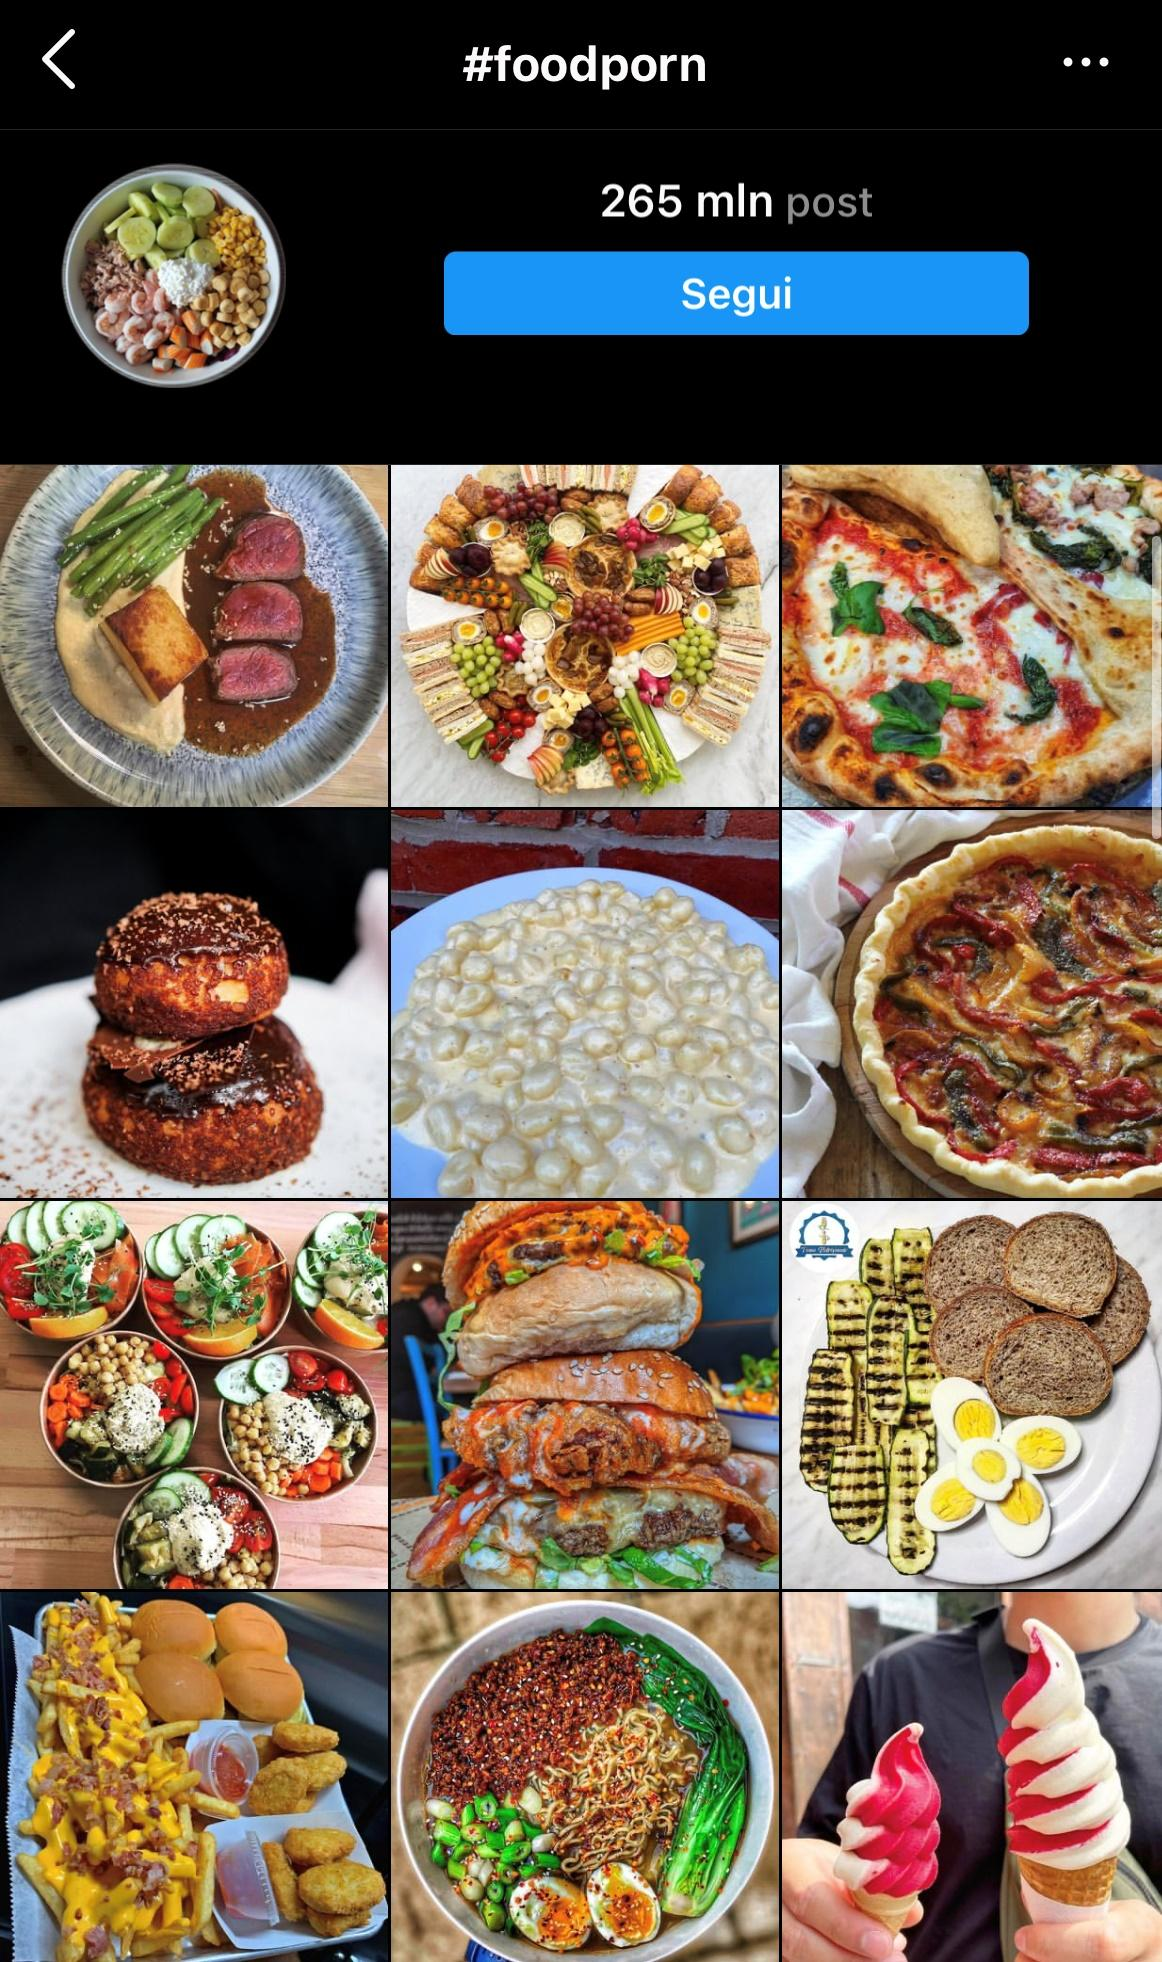
\includegraphics[scale=0.17]{images/foodporn_instagram.jpg}
\caption{Alcune delle 265 milioni di immagini che fanno parte dell'hashtag Foodporn su Instagram}
\label{foodporn}
\end{figure}

Una caratteristica comune delle immagini appartenenti a questo hashtag è che esse evocano nell'utente voglia di assaporare quei cibi, inoltre si è osservato che i cibi poco salutari e i dolci spesso diventano popolari sui social network poiché quelli salutari vengono percepiti dalle persone come meno gustosi, infatti nel 2016 si è visto che all'interno di \#foodporn erano predominanti cibi non salutari \cite{peng2018feast}. 

Generalmente i cibi visibili sui social network o nelle pubblicità tendono anche a diventare dei modelli di estetica a cui i ristoranti cercano di avvicinarsi, cercando sempre più modi per presentare in maniera esteticamente bella i piatti. La presentazione di un piatto gioca un ruolo fondamentale quando si parla della percezione di un utente che lo osserva, in quanto in caso di presentazione del piatto molto articolata o artistica \cite{michel2014taste} gli utenti sono disposti a pagare un prezzo maggiore poiché considerano quel piatto esteticamente bello, molto elaborato e curato. 

Il continuo interesse nella presentazione dei cibi scaturisce dal fatto che il mangiare comincia già con la vista, in particolare il gusto non è solo legato al sapore di un cibo ma dipende anche da tutti gli altri sensi \cite{campo2017effects}. L'aspetto di un cibo ha anche particolari effetti sul corpo umano: viene stimolata la salivazione \cite{wooley1973salivation}, si attivano particolari aree del cervello come l'Amigdala \cite{labar2001hunger} e si creano delle aspettative per quanto riguarda il gusto del cibo stesso. 

Un esempio riguarda il colore \cite{spence2015psychological} del cibo, in particolare se una bevanda è di colore verde si penserà che essa abbia un gusto più aspro rispetto a una bevanda di colore rosso. Inoltre è possibile che anche la forma di un cibo influenzi la nostra percezione \cite{velasco2015hedonic}, un esempio è legato al fatto che la dolcezza viene associata a cibi con forma tondeggiante, mentre forme squadrate o spigolose sono associate cibi salati, amari o aspri.

\section{Outline}
Questa relazione si concentra in primo luogo sulla descrizione dei due dataset utilizzati, ovvero il Gourment Photography Dataset e un dataset creato appositamente, rispettivamente nel Capitolo~\ref{GPD} e nel Capitolo~\ref{new_dataset}. 

Successivamente nel Capitolo~\ref{metodologie} verranno descritti i metodi utilizzati per estrarre le feature usate per le classificazione e nel Capitolo~\ref{risultati} i rispettivi risultati ottenuti. Inoltre sempre nel Capitolo~\ref{metodologie} e nel Capitolo~\ref{risultati} verrà mostrato come visualizzare quali parti di immagine pesano maggiormente per una rete neurale che deve predire la classe di appartenenza di una immagine, dove la classe può essere positiva oppure negativa in base alla valutazione estetica dell'immagine stessa. 

Il Capitolo~\ref{sviluppi}, posto in chiusura della relazione, sarà dedicato alle conclusioni e ai possibili sviluppi futuri del lavoro svolto, individuando eventualmente possibili criticità e punti a favore.





